% IEEE WCNC 2027 submission.
% HARD LIMIT: six (6) printed pages including references. Initial submissions
% longer than six pages are rejected without review. Final versions may run to
% eight, at US$100 per page for pages 7-8.
\documentclass[conference]{IEEEtran}
\IEEEoverridecommandlockouts

\usepackage{cite}
\usepackage{amsmath,amssymb,amsfonts}
\usepackage{graphicx}
\usepackage{booktabs}
\usepackage{multirow}
\usepackage{rotating}
\usepackage{siunitx}
\usepackage[hidelinks]{hyperref}

\sisetup{detect-all, per-mode=symbol}

\begin{document}

\title{The Sidelink Resource Pool, Not the Link Budget,\\
       Limits Hybrid RF/VLC Reliability in Urban V2V}

\author{\IEEEauthorblockN{Eashraque}
\IEEEauthorblockA{\textit{Affiliation} \\
\textit{Institution}\\
City, Country \\
easha003eee@gmail.com}}

\maketitle

\begin{abstract}
% TODO. Write last, once Section V is settled. Roughly 150-200 words.
% Must land: (i) the eV2X 1e-5 row is pool-limited, not link-budget-limited;
% (ii) neither medium alone meets it above rho ~ 17-18; (iii) the optical link
% earns its place by relieving the pool, not by adding diversity -- duplication
% costs twice as much and is eight times worse; (iv) measured over 20.9M
% packets with bootstrap bounds.
\end{abstract}

\begin{IEEEkeywords}
V2V, NR sidelink, visible light communication, resource allocation,
ultra-reliable low-latency communication.
\end{IEEEkeywords}

% ---------------------------------------------------------------------------
\section{Introduction}
\label{sec:intro}
% TODO. Ends with an explicit contributions statement and a roadmap paragraph:
% every WCNC paper surveyed does both. Budget 0.75 page.
%
% Arc: TR 38.913 eV2X row -> hybrid RF/VLC is the standing proposal (cite
% Singh, who targets this exact row with link aggregation) -> prior work models
% the radio as a link, but mode-2 draws from a finite pool and reliability is
% bought with retransmissions that all draw from it -> contributions.

\section{System Model}
\label{sec:system}

We evaluate a hybrid sidelink/optical link against the 3GPP TR~38.913 eV2X
reference row on a microscopic urban mobility model. Both media are exercised
on the same vehicle geometry, so the radio and optical paths available to a
given packet describe the same instant of the same world. Section~\ref{sec:sys:scenario}
describes the scenario, Section~\ref{sec:sys:rf} the sidelink resource model,
Section~\ref{sec:sys:vlc} the optical link, and Section~\ref{sec:sys:obs} what
a transmitter is permitted to observe. Parameters are listed in
Table~\ref{tab:params}.

\subsection{Scenario and Mobility}
\label{sec:sys:scenario}

Vehicles move on a one-way Manhattan grid of $6$ avenues spaced
\SI{244}{\metre} and $12$ cross streets spaced \SI{61}{\metre}, two lanes per
direction, illustrated in Fig.~\ref{fig:scene}. The asymmetric block ratio is
characteristic of the reference topology and is not incidental to the result:
it produces two distinct populations of communicating pairs, long runs along
avenues and short hops between cross streets, whose optical geometry differs
sharply.

All $40$ interior junctions are signalised on a fixed two-phase
\SI{45}{\second} cycle with staggered offsets. Vehicles follow a car-following
law with a \SI{2.5}{\metre} minimum standstill gap, draw from three classes
($90\%$ passenger car, $7\%$ van/SUV, $3\%$ bus/truck) at their configured body
dimensions, and enter at the boundary as a Poisson process tuned to hold one of
three target densities $\rho \in \{10, 20, 30\}$~veh/lane$\cdot$km. Traces
advance at \SI{50}{\milli\second} and are discarded for the first
\SI{300}{\second} so that the seeded formation disperses before measurement.

Signalisation matters for the optical link. The resulting traffic is
stop-and-go rather than free-flowing---median speed \SI{1.2}{\metre\per\second}
with roughly $38\%$ of vehicles stationary at any instant---so following pairs
hold short, stable separations for seconds at a time.


\begin{figure}[t]
  \centering
  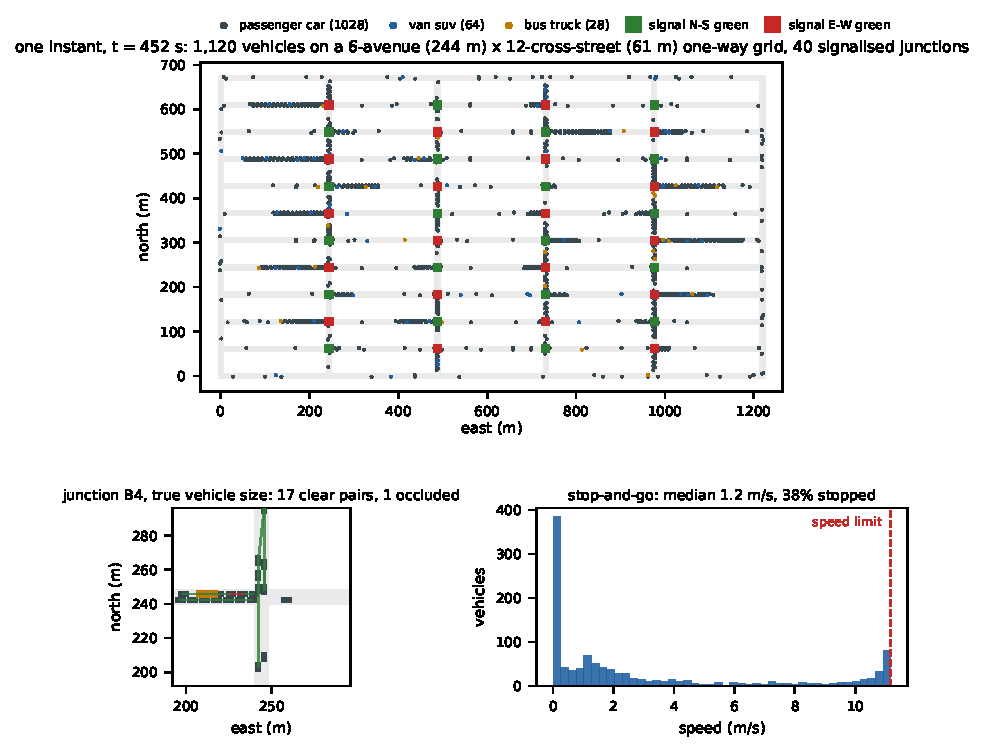
\includegraphics[width=\columnwidth]{figures/fig_traffic_scene.pdf}
  \caption{One instant of the scenario at $\rho = 30$: 1\,120 vehicles on the
  one-way grid with signal phases, and the speed distribution that follows from
  signalisation.}
  \label{fig:scene}
\end{figure}

\subsection{Sidelink Resource Model}
\label{sec:sys:rf}

The radio is NR-V2X mode~2 with sensing-based semi-persistent scheduling. A
vehicle senses the channel, excludes resources it observes to be reserved, and
selects from the remainder. We model the outcome of that procedure rather than
its signalling: a transmission fails when two vehicles select the same
resource, at a rate set by how many contenders there are and how reliably
sensing excludes them.

The quantity that governs the result is the size of the pool they select from.
With $S$ subchannels and a selection window of $W$ slots aligned to the
generation period, the pool offers
\begin{equation}
  M = S \, W
  \label{eq:pool}
\end{equation}
distinct (subchannel, slot) resources per period. For the profile of
Table~\ref{tab:params}, $M = 2 \times 200 = 400$.

Reliability on this link is bought with retransmissions. A packet granted $N$
blind attempts fails only if all $N$ are lost, so with per-attempt failure
probability $q$ and attempts drawn on distinct resources,
\begin{equation}
  p_{\mathrm{RF}} = q^{N}.
  \label{eq:rf}
\end{equation}
Each attempt, however, consumes one resource from the same pool that every
other vehicle draws from. With $n$ contenders in range each claiming $N$
attempts, the population asks for $nN$ of the $M$ that exist. We write this
claim as
\begin{equation}
  D = \frac{nN}{M},
  \label{eq:demand}
\end{equation}
and call the profile \emph{deliverable} only when $D \le 1$.

This is a supply constraint, not a performance one, and it is invisible to the
collision model itself. That model prices where one selection lands; it does
not ask whether every selection can be honoured simultaneously. A profile with
$D > 1$ therefore still reports an ordinary per-attempt failure probability and
a plausible miss rate, both of which describe an assignment that does not
exist. Every reliability figure in Section~\ref{sec:results} is reported
alongside its $D$ for this reason.

Sensing reliability is the one quantity the model declares it does not know
precisely. We carry it as a band---optimistic, nominal and pessimistic---rather
than a point value, and report the verdict on all three.

\subsection{Optical Link}
\label{sec:sys:vlc}

The optical link is vehicle-to-vehicle visible light between a leading
vehicle's tail lamps and a follower's photodiode, at \SI{0.55}{\metre} height
against a \SI{0.7}{\metre} emitter. The emission pattern is a modelled angular
intensity grid fitted so that every UN Regulation~112 Rev.4 Class~B
passing-beam limit is satisfied by construction; it is a regulatory
construction, not a measured lamp, and any optical figure quoted from it
inherits that.

Transmission is on-off keying at a \SI{5}{\mega\hertz} electrical bandwidth,
which is the optimistic edge of what automotive LED junction capacitance
supports. With rate-$1/4$ coding this puts \SI{2.4}{\milli\second} of airtime
on a \SI{300}{\byte} block---roughly five times the \SI{0.5}{\milli\second}
radio slot, a disparity that matters in Section~\ref{sec:results}.

An optical packet fails for one of three reasons: the receiver falls outside
the emitter's field of view, a third vehicle body occludes the path, or the
received signal is too weak for the coded threshold. The first two are
geometric and are decided by the same vehicle positions the radio model reads.
Occlusion is treated as complete: a body intersecting the line of sight
extinguishes the link rather than attenuating it. This is conservative for the
optical leg.

\subsection{Observability}
\label{sec:sys:obs}

Decisions and outcomes are deliberately separated. A transmitter chooses using
cooperative awareness messages---positions perturbed by
$\sigma = \SI{0.5}{\metre}$, delivered with \SI{50}{\milli\second} latency and
aged up to \SI{1}{\second}---while every reported miss rate is computed from
what the channel actually did. A policy that could not have been executed by a
vehicle is therefore visible as such, and Section~\ref{sec:results} states
explicitly which of its results are achievable and which are bounds.

\begin{table}[t]
  \centering
  \caption{Simulation parameters.}
  \label{tab:params}
  \small
  \begin{tabular}{@{}llr@{}}
    \toprule
    & Parameter & Value \\
    \midrule
    \multirow{6}{*}{\rotatebox{90}{Mobility}}
      & Avenues $\times$ cross streets & $6 \times 12$ \\
      & Spacing (avenue, cross street) & $244$, \SI{61}{\metre} \\
      & Lanes per direction & 2 \\
      & Speed limit & \SI{11.18}{\metre\per\second} \\
      & Signal cycle (fixed, two-phase) & \SI{45}{\second} \\
      & Densities $\rho$ & 10, 20, 30 veh/lane$\cdot$km \\
    \midrule
    \multirow{5}{*}{\rotatebox{90}{Sidelink}}
      & Subchannels $S$ & 2 \\
      & Selection window $W$ & 200 slots \\
      & Pool $M = SW$ & 400 per period \\
      & Slot airtime & \SI{0.5}{\milli\second} \\
      & Sensing reliability & 0.70 / 0.85 / 0.95 \\
    \midrule
    \multirow{4}{*}{\rotatebox{90}{Optical}}
      & Modulation & OOK, rate $1/4$ \\
      & Electrical bandwidth & \SI{5}{\mega\hertz} \\
      & Airtime (\SI{300}{\byte} block) & \SI{2.4}{\milli\second} \\
      & Receiver field of view & \SI{60}{\degree} \\
    \midrule
    \multirow{5}{*}{\rotatebox{90}{Service}}
      & Payload & \SI{300}{\byte} \\
      & Generation period & \SI{100}{\milli\second} \\
      & Deadline & \SI{3}{\milli\second} \\
      & Miss budget & $10^{-5}$ \\
      & RF attempts $N$ & 4 \\
    \midrule
    \multirow{3}{*}{\rotatebox{90}{Obs.}}
      & Position noise $\sigma$ & \SI{0.5}{\metre} \\
      & Track latency & \SI{50}{\milli\second} \\
      & Track lifetime & \SI{1}{\second} \\
    \bottomrule
  \end{tabular}
\end{table}

\section{Allocation as a Fixed Point}
\label{sec:allocation}

Suppose some packets are carried optically and never reach the radio. The pool
claim of \eqref{eq:demand} falls, because fewer vehicles contend; the
per-attempt failure probability $q$ falls with it; and $p_{\mathrm{RF}}$
improves for every packet that remains. But whether a packet is worth carrying
optically depends on $p_{\mathrm{RF}}$, which is what just changed. The
allocation and the channel it runs on determine each other, and neither can be
evaluated first.

This section states that circularity as a fixed point and solves it. The
resulting allocation is what Section~\ref{sec:results} evaluates against the
single-medium baselines.

\subsection{Coupling}

Let $f \in [0,1]$ denote the \emph{radio usage fraction}: the share of offered
packets that place a copy on the sidelink. A packet carried optically alone
returns its share of the pool, so three quantities fall together with $f$---the
number of contenders a transmitter competes with, the fraction of the period a
receiver spends transmitting rather than listening, and the pool claim. They are
one behaviour observed three ways and scale from one parameter. The per-attempt
failure probability is written $q(f)$ and the resulting per-packet radio risk
\begin{equation}
  p_{\mathrm{RF}}(f) = q(f)^{N} .
  \label{eq:rf_of_f}
\end{equation}

Half-duplex is why this coupling cannot be approximated away. At the attempt
counts of Table~\ref{tab:params} the half-duplex term is the same order as
collision, so charging a full duty cycle to a receiver that spent the period on
optics overstates radio failure by roughly $1/f$.

\subsection{Per-Packet Allocation}

Given the two risks, the allocation for a population of $K$ packets is the
cheapest assignment of media that meets the budget $\varepsilon$. Each packet
$k$ has a radio risk $p_{\mathrm{RF},k}$ and an optical risk
$p_{\mathrm{VLC},k}$, and may be assigned to the radio alone, the light alone,
or both. Activation costs are $1$, $1$ and $2$ respectively, so the cheapest
single-medium choice is whichever leg is less likely to fail,
\begin{equation}
  \pi_k = \min\!\left(p_{\mathrm{RF},k},\; p_{\mathrm{VLC},k}\right),
  \label{eq:single}
\end{equation}
and duplication is an upgrade that costs one further activation and, assuming
independence across media, reduces the packet's risk to
$p_{\mathrm{RF},k}\,p_{\mathrm{VLC},k}$.

Minimising mean cost subject to
$K^{-1}\sum_k \pi_k \le \varepsilon$ is then a linear relaxation whose solution
is greedy: baseline every packet on its cheaper leg, and upgrade packets to
duplication in decreasing order of the risk each upgrade removes,
\begin{equation}
  \Delta_k = \pi_k - p_{\mathrm{RF},k}\,p_{\mathrm{VLC},k},
  \label{eq:reduction}
\end{equation}
stopping as soon as the budget is met. Two properties of this rule matter
later. It can \emph{substitute}, not only duplicate---a packet whose optical
path is clean is routed to the light and off the radio entirely, which is what
relieves the pool---and it returns a mean activation cost, so the price of
meeting the budget is reported rather than assumed.

Independence across media is assumed in the $p_{\mathrm{RF}}p_{\mathrm{VLC}}$
term. The campaign measures the realised joint failure at a dependence ratio of
$1.18$ at $\rho = 30$, so the true joint outcome is slightly worse than
independence predicts and the duplication branch is correspondingly optimistic.
The allocation branch, which is the one that carries the result, does not use
that term.

\subsection{Solution}

Writing $\mathcal{A}$ for the allocation of \eqref{eq:single}--\eqref{eq:reduction}
and $f = \mathcal{A}\!\left(p_{\mathrm{RF}}(f), p_{\mathrm{VLC}}\right)$ for the
radio usage it induces, an operating point is a solution of
\begin{equation}
  f^{\star} = \mathcal{A}\!\left(p_{\mathrm{RF}}(f^{\star}),\, p_{\mathrm{VLC}}\right).
  \label{eq:fixedpoint}
\end{equation}
We solve \eqref{eq:fixedpoint} by damped iteration,
$f_{i+1} = (1-\lambda) f_i + \lambda \, \mathcal{A}(p_{\mathrm{RF}}(f_i), p_{\mathrm{VLC}})$,
with $\lambda = 0.25$.

Damping is not cosmetic. Undamped, the iteration oscillates at the higher
attempt counts: offloading improves the radio, which makes offloading
unattractive, which congests it again. That oscillation is an artefact of
updating every vehicle simultaneously---a real fleet decides asynchronously,
and $\lambda$ is what represents that.

Two properties of \eqref{eq:fixedpoint} require care.

\emph{The map has more than one fixed point.} Started from full radio use, a
congested pool makes duplication look necessary and duplicating keeps it
congested; the iteration settles there, self-consistently, at cost $2.0$ and a
miss rate that fails the budget. Started lower, the same inputs settle on most
packets going by light, the offered load collapsing, and the radio comfortably
carrying the remainder at cost $1.0$. Both are equilibria of the same system,
and at $\rho = 30$ on the pessimistic band they differ by a factor of $325$. We
therefore sweep several starting loads and report the cheapest feasible
equilibrium found, together with how many distinct equilibria were reached.
Bistability here is a property of the system rather than of the solver: a fleet
that begins congested stays congested absent something to coordinate the move
to light.

\emph{An exact fixed point need not exist.} The allocation is a discrete
ordering over a finite packet population, so $\mathcal{A}$ is a step function
and $\mathcal{A}(f) = f$ may have no solution. What exists is a small invariant
band. We therefore declare convergence on the reported quantities---the miss
rate and the mean cost---rather than on $f$ itself, which is what a published
number requires and what a stationarity test on a step function never delivers.

\subsection{Relation to Prior Fixed-Point Analyses}

Fixed-point analysis of C-V2X contention is established: Wang \emph{et al.}
solve one for semi-persistent scheduling, in which collision probability
depends on the idle resources a vehicle can sense, which in turn depend on the
collision probability~\cite{wang2018fixedpoint}. That fixed point is in the
collision probability \emph{at a fixed offered load}. The fixed point of
\eqref{eq:fixedpoint} is in the \emph{allocation}---in how much load leaves the
radio altogether---and it is the pool constraint \eqref{eq:demand}, absent from
single-medium analyses, that gives that departure its value.

\section{Results}
\label{sec:results}
% TODO. Blocked on the realizability framing decision. Budget 1.75 pages,
% three figures: pool ceiling, feasibility boundary, and one of the frontier or
% the realizable-selector table.

\section{Conclusion}
\label{sec:conclusion}
% TODO. Budget 0.25 page. State limitations plainly, as the surveyed papers do:
% synthetic mobility, binary occlusion, single beam variant, and whichever
% realizability position Section IV takes.


\bibliographystyle{IEEEtran}
\bibliography{refs}

\end{document}
